\section{预备知识:Kan延拓}
回顾一下\cite{李文威卷二}中关于Kan延拓的说明.
\begin{definition}[Kan延拓]\label{Def:Kan延拓}
    考虑范畴$\mathcal{C,D,E}$间的图表
    \[\begin{tikzcd}
	{\mathcal{C}} \\
	{\mathcal{D}} & {\mathcal{E}}
	\arrow["K"', from=1-1, to=2-1]
	\arrow["F", curve={height=-10pt}, from=1-1, to=2-2]
    \end{tikzcd}\]
    其中$K : \mathcal{C} \to \mathcal{D}$, $F: \mathcal{C} \to \mathcal{E}$.
    \begin{itemize}
        \item 函子$F$沿$K$的左Kan延拓意谓以下资料$(\Lan_K F,\eta)$,其中
        \begin{itemize}
            \item $\Lan_KF: \mathcal{D} \to \mathcal{E}$是函子.
            \item $\eta : F\to (\Lan_K F)K$是函子间的态射.
        \end{itemize}
        使得以下泛性质成立:对任何资料$L :\mathcal{D} \to \mathcal{E}$,和$\xi : F \to LK$,存在唯一的态射$\chi: \Lan_K F \to L$使得$\xi = (\chi K)\eta$(态射的纵横合成),或以2-胞腔图解为
        \[\begin{tikzcd}
	{\mathcal{C}} \\
	{\mathcal{D}} & {\mathcal{E}}
	\arrow["K"', from=1-1, to=2-1]
	\arrow[""{name=0, anchor=center, inner sep=0}, "F", curve={height=-12pt}, from=1-1, to=2-2]
	\arrow["L"', from=2-1, to=2-2]
	\arrow["\xi"{description}, shorten <=4pt, Rightarrow, from=0, to=2-1]
        \end{tikzcd}=
        \begin{tikzcd}
	{\mathcal{C}} \\
	{\mathcal{D}} & {\mathcal{E}}
	\arrow["K"', from=1-1, to=2-1]
	\arrow[""{name=0, anchor=center, inner sep=0}, "F", curve={height=-12pt}, from=1-1, to=2-2]
	\arrow[""{name=1, anchor=center, inner sep=0}, "{\Lan_K F}"', from=2-1, to=2-2]
	\arrow[""{name=2, anchor=center, inner sep=0}, "L"', curve={height=30pt}, from=2-1, to=2-2]
	\arrow["\eta"{description}, shorten <=4pt, Rightarrow, from=0, to=2-1]
	\arrow["\chi", shorten <=7pt, shorten >=2pt, Rightarrow, from=1, to=2]
    \end{tikzcd}\]
    \item 函子$F$沿$K$的右延拓意谓以下资料$(\Ran_K F , \varepsilon)$,其中
    \begin{itemize}
        \item $\Ran_K F: \mathcal{D} \to \mathcal{E}$是函子.
        \item $\varepsilon: (\Ran_K F)K \to F$是函子间的态射.
    \end{itemize}
    使得以下泛性质成立:对任何资料$R : \mathcal{D} \to \mathcal{E}$和$\delta : RK \to F$,存在唯一的$\theta : R \to (\Ran_KF)K$使得$\delta = \varepsilon(\theta K)$,或用2-胞腔图解为
    \[\begin{tikzcd}
	{\mathcal{C}} \\
	{\mathcal{D}} & {\mathcal{E}}
	\arrow["K"', from=1-1, to=2-1]
	\arrow[""{name=0, anchor=center, inner sep=0}, "F", curve={height=-12pt}, from=1-1, to=2-2]
	\arrow["R"', from=2-1, to=2-2]
	\arrow["\delta"{description}, shorten >=4pt, Rightarrow, from=2-1, to=0]
\end{tikzcd}=\begin{tikzcd}
	{\mathcal{C}} \\
	{\mathcal{D}} & {\mathcal{E}}
	\arrow["K"', from=1-1, to=2-1]
	\arrow[""{name=0, anchor=center, inner sep=0}, "F", curve={height=-12pt}, from=1-1, to=2-2]
	\arrow[""{name=1, anchor=center, inner sep=0}, "{\Ran_K F}"', from=2-1, to=2-2]
	\arrow[""{name=2, anchor=center, inner sep=0}, "R"', curve={height=30pt}, from=2-1, to=2-2]
	\arrow["\varepsilon"{description}, shorten >=4pt, Rightarrow, from=2-1, to=0]
	\arrow["\theta", shorten <=2pt, shorten >=7pt, Rightarrow, from=2, to=1]
    \end{tikzcd}\]
    \end{itemize}
\end{definition}
\begin{proposition}\label{Pro:Kan延拓定义}
    给定范畴$\mathcal{C},\mathcal{D},\mathcal{E}$和函子$K : \mathcal{C} \to \mathcal{D}$, $F :\mathcal{C} \to \mathcal{E}$.考虑拉回函子$K^* \mathcal{E}^{\mathcal{D}} \to \mathcal{E}^{\mathcal{C}}$.
    \begin{enumerate}
        \item 精确到$\mathcal{E}^{\mathcal{D}}$中唯一的同构,左Kan延拓$(\Lan_KF,\eta)$若存在则唯一;右Kan延拓亦是如此.
        \item 若沿$K$的左Kan延拓(或右Kan延拓)对所有$F$皆存在,则得到$K^*$的左伴随函子$\Lan_K : \mathcal{E}^{\mathcal{D}}\to \mathcal{E} \to \mathcal{C}$(或右伴随函子$\Ran_K : \mathcal{E}^{\mathcal{D}}\to \mathcal{E} \to \mathcal{C}$),定义\ref{Def:Kan延拓}中$\eta$(或$\varepsilon$)所构成的态射族正是伴随对中单位(余单位)态射.
    \end{enumerate}
\end{proposition}
\begin{proof}
    显然.
\end{proof}
\begin{remark}
    有些教材直接使用这个命题作为Kan延拓定义.
\end{remark}
发现Kan延拓其实是在寻求一个$G : \mathcal{D} \to \mathcal{E}$使得$F$与$GK$之间有一个最佳的逼近.那么如何对于$d \in \Obj(\mathcal{D})$定义$Gd$就成了问题.唯一的线索是当$d = Kc$时, $Gd$在同构意义下应当被取为$Fc$.因此可以使用所有的$Fc$的$\indlim$(或$\prolim$)来逼近$Gd$,极限取遍所有的$c \in \Obj(\mathcal{C})$和态射$Kc \to d$(或$d \to Kc)$.为了记号上的方便,对于俯仰范畴进行一个扩充,得到以下定义.\footnote{其实是\parencite[定义1.6.2]{李文威卷二}}
\begin{definition}
    若$F : \mathcal{C} \to \mathcal{D}$为函子,且$d \in \mathcal{D}$为一个对象.定义$F_{/d}$为拉回
    \[\begin{tikzcd}
	{F_{/d}} & {\mathcal{D}_{/d}} \\
	{\mathcal{C}} & {\mathcal{D}}
	\arrow[from=1-1, to=1-2]
	\arrow[from=1-1, to=2-1]
	\arrow[from=1-2, to=2-2]
	\arrow["F", from=2-1, to=2-2]
    \end{tikzcd}\]
    即$F_{/d}$中对象为$(c\in \mathcal{C},\alpha : F(c) \to d)$态射为使得以下图表交换的$\beta$
    \[\begin{tikzcd}
	{F(c)} && {F(c')} \\
	& d
	\arrow["{F(\beta)}", from=1-1, to=1-3]
	\arrow["\alpha"', from=1-1, to=2-2]
	\arrow["{\alpha'}", from=1-3, to=2-2]
    \end{tikzcd}\]
    当$F$为子范畴的嵌入函子时,简写为$\mathcal{C}_{/d}$,类似定义$F_{d/}$和$\mathcal{C}_{d/}$.\\
    可以发现$F_{/d}$(或$F_{d/}$)带有典范的投影函子$\prod_{/d}: F_{/d} \to \mathcal{C}$将$(c,\alpha: F(c) \to d)$(或$(c,\alpha:d \to F(c))$)映为$c$,态射$\beta$映为$\beta$.
\end{definition}
今后的重点在于合成函子$F \prod_{/d}: K_{/d} \to \mathcal{E}$和$F\prod_{d/}: K_{d/} \to \mathcal{E}$,它们分别映对象$(c,Kc \to d)$和$(c,d \to Kc)$为$Fc$.在极限存在的情况下,可以做几点观察:
\begin{itemize}
    \item 任何$d \to d'$诱导典范态射$\indlim F\prod_{/d} \to \indlim F \prod_{/d'}$;其刻画为使得图表
    \[\begin{tikzcd}
	Fc & Fc \\
	{\indlim F\prod_{/d}} & {\indlim F\prod_{/d'}}
	\arrow[shift left, no head, from=1-1, to=1-2]
	\arrow[shift right, no head, from=1-1, to=1-2]
	\arrow[from=1-1, to=2-1]
	\arrow[from=1-2, to=2-2]
	\arrow[from=2-1, to=2-2]
    \end{tikzcd}\]
    对每个$(c,Kc \to d)\in \Obj(K_{/d})$交换(它诱导$(c,Kc \to d') \in \Obj(K_{/d'})$),纵向箭头即为$\indlim$自带的典范态射.
    \item 考虑$(c,Kc \xrightarrow{\identity} Kc)\in \Obj(K_{/Kc})$得到典范态射$\eta_c : Fc \to \indlim F\prod_{/Kc}$.
    \item 任何$c \to c'$皆诱导典范态射$\indlim F\prod_{/Kc}   \to \indlim F\prod_{/Kc'}$使得
    \[\begin{tikzcd}
	Fc & {Fc'} \\
	{\indlim F\prod_{/Kc}} & {\indlim F\prod_{/Kc'}}
	\arrow[from=1-1, to=1-2]
	\arrow[from=1-1, to=2-1]
	\arrow[from=1-2, to=2-2]
	\arrow[from=2-1, to=2-2]
    \end{tikzcd}\]
    交换.鉴于对偶性,$\prolim F\prod_{d/}$也具备相应性质,如典范态射$\varepsilon_c : \prolim F \prod_{Kc/} \to Fc$等等.次一定理的陈述基于这些函子性.
\end{itemize}
\begin{theorem}\label{The:Kan延拓逐点构造}
考虑函子$K :\mathcal{C} \to \mathcal{D}$和$F : \mathcal{C}  \to \mathcal{E}$.
    \begin{enumerate}
        \item 若对于每个$d\in \Obj(\mathcal{D})$,极限$\indlim(F\prod_{/d})$在$\mathcal{E}$中存在,则$(\Lan_K F)(d) := \indlim (F\prod_{/d})$连同前文对应的交换图表给出的函子性确定了左Kan延拓$\Lan_K F : \mathcal{D} \to \mathcal{E}$,相应$\eta : F \to (\Lan_K F)K$来自于前文讨论的$(\eta_c)_{c\in \Obj(\mathcal{C})}$.
        \item 若对于每个$d\in \Obj(\mathcal{D})$,极限$\prolim(F\prod_{d/})$在$\mathcal{E}$中存在,则$(\Ran_K F)(d) := \prolim (F\prod_{d/})$连同函子性确定了右Kan延拓$\Ran_K F : \mathcal{D} \to \mathcal{E}$,相应$\varepsilon : (\Ran_KF )K  \to F$来自于前文讨论的$(\varepsilon_c)_{c\in \Obj(\mathcal{C})}$.
        \item 若$K: \mathcal{C} \to \mathcal{D}$全忠实,则$\eta$与$\varepsilon$同构.
    \end{enumerate}
\end{theorem}
\begin{proof}
    \begin{enumerate}
        \item[1.与2.]由于1.与2.是对偶的,因此只需要证明1.的情况,这无非是依照泛性质验证Kan延拓定义,对于$L: \mathcal{D} \to \mathcal{E}$以及$\xi : F \to LK$利用归纳极限的泛性质得知存在$\chi_d : (\Lan_K F )(d) \to Ld$,具体刻画为图表
        \[\begin{tikzcd}
	Fc & {(\Lan_L F)(d)} \\
	LKc & Ld
	\arrow[from=1-1, to=1-2]
	\arrow["{\xi_c}"', from=1-1, to=2-1]
	\arrow["{\chi_d}", from=1-2, to=2-2]
	\arrow["{L(Kc \to d)}"', from=2-1, to=2-2]
        \end{tikzcd}\]
        其自然给出$\chi : \Lan_K F \to L$.根据$\chi_d$定义可以得知$\xi_c = \chi_{Kc}\eta_c : Fc \to LKc$.这图表中取$d = Kc$即可. $\chi$的唯一性也是容易的.因此得知$\Lan_K F$确实为左Kan延拓.
        \item[3.] 取定$c\in \Obj(\mathcal{C})$.由$K$的全忠实性可知$K_{/Kc}$有终对象$(c, Kc \xrightarrow{\identity} Kc)$,而$\eta : Fc \to \indlim F \prod_{/Kc}$来自于此终对象,故为同构.
    \end{enumerate}
\end{proof}
\begin{remark}\label{Rk:拉回函子左右伴随}
    若$\mathcal{C}$为小范畴,则$K_{/d}$和$K_{d/}$对每个$d \in \Obj(\mathcal{D})$都是小范畴.因此当$\mathcal{E}$余完备(或完备)时,命题\ref{Pro:Kan延拓定义}与定理\ref{The:Kan延拓逐点构造}可以说明拉回函子$K^*$必有左伴随(或右伴随).
\end{remark}
引入Kan延拓可以证明一个在单纯集中常常用到的性质.
为此,我们先证明一个引理
\begin{lemma}[米田嵌入的稠密性]\label{Lem:米田嵌入的稠密性}
    每个预层都可以被表现为代表元的归纳极限.更精确地说,每个预层$\mathcal{F} :\mathcal{C}^{\opposite} \to \Set$.典范态射
    \[
    \underset{X\in \mathcal{C}_{/\mathcal{F}}}{\indlim}{h_X} \to \mathcal{F}
    \]
    为同构.其中$\mathcal{C}_{/\mathcal{F}}$为范畴到其预层范畴的Yoneda嵌入所诱导的切片范畴.
\end{lemma}
\begin{proof}
    观察到对于任意预层$\mathcal{G}$都有
    \[
    \Hom_{\mathcal{C}^{\land}}(\underset{X\in \mathcal{C}_{/\mathcal{F}}}{\indlim}h_X,\mathcal{G}) \simeq \underset{X\in \mathcal{C}_{/\mathcal{F}}}{\prolim}\Hom_{\mathcal{C}^{\land}}(h_X,\mathcal{G})
    \]
    而后应用Yoneda引理得到
    \[
    \underset{X\in \mathcal{C}_{/\mathcal{F}}}{\prolim}\Hom_{\mathcal{C}^{\land}}(h_X,\mathcal{G})\simeq \underset{X\in \mathcal{C}_{/\mathcal{F}}}{\prolim} \mathcal{G}(X).
    \]
    而后者无非是$\mathcal{F}$到$\mathcal{G}$的全体自然变换.因此$\Hom_{\mathcal{C}^{\land}}(\underset{X\in \mathcal{C}_{/\mathcal{F}}}{\indlim}h_X,\mathcal{G})\simeq \Hom_{\mathcal{C}^{\land}}(\mathcal{F},\mathcal{G})$由Yoneda引理自然推知引理成立.
\end{proof}
\begin{remark}\label{Rk:嵌入的Kan延拓}
    考虑嵌入函子的拉回:$\iota^{*} : \mathcal{D}^{\mathcal{E}}\to \mathcal{D}^{\mathcal{C}_0}$其中$\mathcal{C}_0\subset \mathcal{C}$为(小)范畴,且$\mathcal{D}$是双完备的\footnote{即完备且余完备.}.根据注记\ref{Rk:拉回函子左右伴随}知其左右伴随(Kan延拓)均存在,分别记为$\iota_!$和$\iota_*$.逐点构造得到
    \begin{align*}
        \iota_!(\mathcal{F})(d) &= \underset{c\in (\mathcal{C}_0)_{/d}}{\indlim} \mathcal{F}(c)\\
        \iota_*(\mathcal{F})(d) & = \underset{c\in (\mathcal{C}_0)_{d/}}{\prolim}\mathcal{F}(c).
    \end{align*}
\end{remark}
可以发现引理\ref{Lem:米田嵌入的稠密性}事实上在说$\iota_!(\mathcal{F}) = \mathcal{F}$.即沿着Yoneda嵌入的左Kan延拓为$\mathcal{C}^{\land}$的恒等函子.


\section{覆叠映射与 Serre 纤维化}
现在我们把覆叠映射概念通过 Kan 纤维化推广到单纯集上,回忆到在拓扑空间中一个映射$f : X\to S$,若对任意$s\in S$都存在一个开邻域$U \subset S$使得$f^{-1}(U)$同胚于若干个$U$的无交并,或者说$f^{-1}(U) = \bigcup_{i\in I}U_i$其中$U_i \simeq U$为同胚.\\
若我们需要将这一概念推广到单纯集上,我们需要将拓扑空间上的 Serre 纤维化与 Kan 纤维化产生联系.
\begin{definition}
    令$q: X \to S$为拓扑空间之间的连续函数.若对于$n \in \Z_{\geq 0}$, $\{0\}\times |\Delta^n| \hookrightarrow [0,1]\times |\Delta^n|$都具有右提升性质,即以下图表中提升存在
    \[\begin{tikzcd}
	{\{0\}\times |\Delta^n|} & X \\
	{[0,1]\times |\Delta^n|} & S
	\arrow[from=1-1, to=1-2]
	\arrow[from=1-1, to=2-1]
	\arrow["q", from=1-2, to=2-2]
	\arrow[dashed, from=2-1, to=1-2]
	\arrow[from=2-1, to=2-2]
    \end{tikzcd}\]
    则称$q$为 Serre 纤维化.
\end{definition}
\begin{example}
    \begin{itemize}
        \item 每个 Hurewicz 纤维化(假定读者都知道 Hurewicz 纤维化,或见\href{https://ncatlab.org/nlab/show/Hurewicz+fibration}{nlab})都是 Serre 纤维化.
        \item 对于任意拓扑空间$X$, $X \to \{\point\}$是 Serre 纤维化.
    \end{itemize}
\end{example}
\begin{proposition}
    令$q: X \to S$为拓扑空间之间的连续映射则其为 Serre 纤维化当且仅当 $\Sing(q)$为 Kan 纤维化.
\end{proposition}
\begin{proof}
    见\cite{Kerodon}[\href{https://kerodon.net/tag/021V}{021V}].
\end{proof}
\begin{definition}
    令$f:X \to S$为单纯集之间的态射,若对于$0\leq j \leq n$以及$n\in \Z_{\geq 1}$都存在唯一的提升
    \[\begin{tikzcd}
        {\Lambda_j^n} & X \\
	{\Delta^n} & S
	\arrow[from=1-1, to=1-2]
   \arrow[hook, from=1-1, to=2-1]
	\arrow["f", from=1-2, to=2-2]
	\arrow[dashed, from=2-1, to=1-2]
	\arrow[from=2-1, to=2-2]
    \end{tikzcd}\]
    使得图表交换,则称$f$为覆叠映射.
\end{definition}
\begin{remark}
    \begin{itemize}
        \item 令$\delta_f : X \to X\dtimes{S} X$为相对于$f$的对角态射,则$f$为覆叠映射当且仅当$f$和$\delta_f$均为 Kan 纤维化.特别地,每个覆叠映射都是 Kan 纤维化.
        \item 覆叠映射关于拉回稳定(验证!).
        \item 覆叠映射关于态射复合稳定.
        \item 考虑交换图表
        \[\begin{tikzcd}
        A & X \\
	B & S
	\arrow[from=1-1, to=1-2]
	\arrow["i"', from=1-1, to=2-1]
	\arrow["f", from=1-2, to=2-2]
	\arrow[dashed, from=2-1, to=1-2]
	\arrow[from=2-1, to=2-2]
        \end{tikzcd}\]
        态射$f$为覆叠映射当且仅当在$i$为平淡态射时,上图中提升唯一存在.
    \end{itemize}
\end{remark}
接下来,我们讨论单纯集的覆叠映射与拓扑空间中覆叠映射的关联.
\begin{proposition}
    若$f:X\to S$为拓扑空间之间的覆叠映射.则其诱导的奇异单纯集$\Sing(f):\Sing(X) \to \Sing(S)$为单纯集之间的覆叠映射.
\end{proposition}
\begin{proof}
    只需要验证$\Sing(\delta_f)$以及$\Sing(f)$均为 Kan 纤维化即可.首先令$\delta_f: X \to X\dtimes{S}X$为相对于$f$的对角态射.只需要说明$\delta_f$将$X$视为$X\dtimes{S} X$在拓扑空间范畴中的的直和项(即其为$X$到$X\dtimes{S} X$上既开又闭子集的一个同胚)即可,这只需要局部地对于$S$进行考虑,从而约化为$S$为离散拓扑空间的情况,此时由覆叠映射定义可知显然成立.因此其诱导的态射
    \[
        \Sing(\delta_f) : \Sing(X) \hookrightarrow \Sing(X\dtimes{S} X)\simeq \Sing(X) \dtimes{\Sing(S)}\Sing(X)
    \]
    为直和项的嵌入,因此由例\ref{例:Kan 纤维化}即知$\Sing(\delta_f)$为 Kan 纤维化,而后验证$\Sing(f)$的情况,由代数拓扑学知识(\cite{TomDieck} Theorem 3.2.2.)我们可以知道覆叠映射为 Hurewicz 纤维化因此自然为 Serre 纤维化,因此 $\Sing(f)$ 自然为 Kan 纤维化.
\end{proof}
\begin{proposition}
    若$f:X \to S$为单纯集之间的覆叠映射,则几何实现$|f|: |X| \to |S|$为拓扑空间之间的覆叠映射.
\end{proposition}
\section{基点与同伦范畴}

\subsection{基点与同伦范畴}
所谓带基点的空间(后简称为带点空间)定义为二元组$(X,*)$其中$*$为一个空间而$*$为其内一点(即所谓基点),一般把基点记为$*$,当然也可以使用其它符号.我们会对于基点的选择加以限制:譬如要求$\{*\}$为闭集.\\
现在考虑带基点的紧生成空间所构成的范畴$\cate{CG}_{*}$,其间态射为保持基点的态射.这个范畴是完备且余完备的.我们可以如下构造其积
\[
 (X,*)\times (Y,*) \simeq (X\times Y,(*,*))
\]
余积刻画为楔(xi\={e})和(或称约化余积)
\[
X \lor Y = \frac{X\sqcup Y}{*_X \sim *_Y}
\]
在$\cate{CG}_*$中,单点空间$*$是始对象以及终对象.可以看出,$\cate{CG}_*$不是 Cartesian 闭的.但是可以在其中取出``映射对象'':定义$Y^{X}_*$为$Y^X$中由保持基点的态射所构成的子空间.由于$\{*\}$是闭的,因此$Y_*^X$在$Y^X$中是闭的,即它确实是紧生成空间.既然无法要求 Cartesian 闭,我们退而求其次考虑是否可以定义一个双函子$-\otimes -$使得$(-)^{X}_*$为$\underline{\Hom}(X,-)$.不难发现
\[\begin{tikzcd}
	{\Hom_{\cate{CG}}(W,Y^X)} & {\{f: W \times X \to Y\}} \\
	{\Hom_{\cate{CG}}(W,Y^X_*)} & {\{f:f(w,*)=*,\forall w\in W\}} \\
	{\Hom_{\cate{CG}_*}(W,Y^X_*)} & \begin{array}{c} \left\{f\left|\substack{f(w,*) = *,\forall w\in W\\f(*,x) = *,\forall x\in X}\right.\right\} \end{array}
	\arrow["{=}"{marking, allow upside down}, draw=none, from=1-1, to=1-2]
	\arrow["\subset"{marking, allow upside down}, draw=none, from=2-1, to=1-1]
	\arrow["{=}"{marking, allow upside down}, draw=none, from=2-1, to=2-2]
	\arrow["\subset"{marking, allow upside down}, draw=none, from=2-2, to=1-2]
	\arrow["\subset"{marking, allow upside down}, draw=none, from=3-1, to=2-1]
	\arrow["{=}"{marking, allow upside down}, draw=none, from=3-1, to=3-2]
	\arrow["\subset"{marking, allow upside down}, draw=none, from=3-2, to=2-2]
\end{tikzcd}\]
因此可以发现映射$W \times X \to Y$对应的$f : W \to Y^X_*$将楔和$W\lor W\subset X \times W$缩为$Y$的基点,从而唯一穿过缩积
\[
W\land X = \frac{W\times X}{W\lor X}
\]
可以得到伴随对
\[
-\land X : \cate{CG}_*\leftrightarrows : \cate{CG}_* : (-)_*^X.
\]
一个很好的造出带基点空间的方式是考虑二元组$(X,A)$其中$A\subset X$为闭子空间,而后将$A$缩为一点.因此
\[
\Hom_{\cate{CG}_*}(X/A,Y) = \{f:X \to Y : f(A)\subset \{*\}\}
\]
当$A = \varnothing$时.
\[
 \Hom_{\cate{CG}_*}(X/\varnothing,Y) = \Hom_{\cate{Top}}(X,uY)
\]
其中$uY$表示遗忘基点后的$Y$.其解为$X$无交并上一个基点.记为$X/\varnothing = X_+$.这个时候给出了另一对伴随$(-)_+\dashv u$.\\
对于$A\subset X$与$B\subset Y$有
\[
(X/A) \land (Y/B) = \frac{X\times Y}{(A\times Y) \dsqcup{A\times B}(X\times B)}
\]
这样的缩积是非常有用的,比如说我们在考虑$I^m/\partial I^m$作为$S^m$视为带基点的空间的模型时,可以发现
\[
S^m \land S^n =(I^m/\partial I^m)\land(I^n /\partial I^n) = \frac{I^{m+n}}{(\partial I^m\times I^n)\dsqcup{\partial I^m \times \partial I^n}(I^m \times \partial I^n)}
\]
$(\partial I^m\times I^n)\dsqcup{\partial I^m \times \partial I^n}(I^m \times \partial I^n)$即为$\partial I^{m+n}$.因此$S^m \land S^n = S^{m+n}$.\\
在同伦论中,一个重要构造是与$S^1$的缩积,又称为(约化)纬悬:
\[
    \Sigma X = S^1 \land X = \frac{I\times X}{(\partial I \times X) 
    \cup (I\times *)}
\]
我们通过下例来给出$\Sigma X$的直观.
\begin{example}
    考虑拓扑空间$X$,记其双锥为$SX$,直观如下\footnote{图来自香蕉空间.}
    \[
    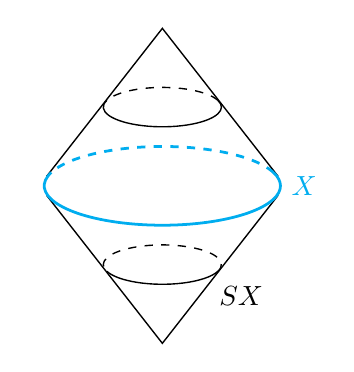
\begin{tikzpicture}
        \draw [line width = .5] (-1.47, .12) -- (0, 2) -- (1.47, .12) (-1.47, -.12) -- (0, -2) -- (1.47, -.12);
        \draw [line width = 1, cyan, dashed] (20:1.5 and .5) arc (20:160:1.5 and .5);
        \draw [line width = 1, cyan] (160:1.5 and .5) arc (160:380:1.5 and .5);
        \draw [line width = .5, dashed] (0, 1) + (20:.75 and .25) arc (20:160:.75 and .25);
        \draw [line width = .5] (0, 1) + (160:.75 and .25) arc (160:380:.75 and .25);
        \draw [line width = .5, dashed] (0, -1) + (-20:.75 and .25) arc (-20:200:.75 and .25);
        \draw [line width = .5] (0, -1) + (200:.75 and .25) arc (200:340:.75 and .25);
        \node [cyan] at (1.8, 0) {$X$};
        \node at (1, -1.4) {$S X$};
    \end{tikzpicture}
    \]
    其约化纬悬为在双锥$SX$中将基点$*$所对应的母线压缩为一点,从而得到新的基点,直观如下
    \[
    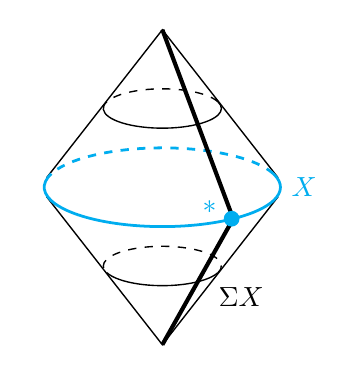
\begin{tikzpicture}
        \draw [line width = .5] (-1.47, .12) -- (0, 2) -- (1.47, .12) (-1.47, -.12) -- (0, -2) -- (1.47, -.12);
        \draw [line width = 1, cyan, dashed] (20:1.5 and .5) arc (20:160:1.5 and .5);
        \draw [line width = 1, cyan] (160:1.5 and .5) arc (160:380:1.5 and .5);
        \draw [line width = .5, dashed] (0, 1) + (20:.75 and .25) arc (20:160:.75 and .25);
        \draw [line width = .5] (0, 1) + (160:.75 and .25) arc (160:380:.75 and .25);
        \draw [line width = .5, dashed] (0, -1) + (-20:.75 and .25) arc (-20:200:.75 and .25);
        \draw [line width = .5] (0, -1) + (200:.75 and .25) arc (200:340:.75 and .25);
        \draw [line width = 1.5] (0, 2) -- (.9, -.4) -- (0, -2);
        \fill [cyan] (.88, -.4) circle (.1);
        \node [cyan] at (1.8, 0) {$X$};
        \node [cyan] at (.6, -.25) {$*$};
        \node at (1, -1.4) {$\Sigma X$};
    \end{tikzpicture}
    \]
    由此不难看出纬悬实际上是一种自然的将空间提高一维的方法.
\end{example}
\begin{proposition}\label{命题:缩积的性质}
    缩积具有以下性质(此处将缩积类比于幺半范畴的张量积函子)
    \begin{enumerate}
        \item 它具有函子性.
        \item 双点空间$S^0=\{0,1\}$(其中$0$为基点)与任何空间$X$的缩积为$X$自身,换言之,双点空间在缩积运算中为单位元.
        \item 在$\cate{CG}_*$中缩积满足结合律以及交换律.
    \end{enumerate}
\end{proposition}
\begin{proof}
    只需要对于结合律进行验证即可,其它的都是平凡的.对于结合律,只需说明$(X\land Y) \land Z$和$X\land(Y \land Z)$实际上为$(X\times Y \times Z)/A$即可,其中
    \[
    A = \{(x,y,z)\in X \times Y \times Z: x= *_X \text{或} y = *_Y \text{或} z = *_Z\}
    \]
\end{proof}
事实上,缩积在$\cate{Top}$中不一定服从结合律.由命题\ref{命题:缩积的性质}可逐步归纳出$n$-重纬悬,即
\[
 \Sigma^n X = S^1 \land \Sigma^{n-1}X = S^1\land(S^{n-1}\land X) = (S^{1}\land S^{n-1})\land X = S^n \land X
\]
此外,命题\ref{命题:缩积的性质}也说明缩积给出$\cate{CG}_*$上的闭对称幺半结构.\\
此外,可以研究带点空间的环路空间,它定义为
\[
    \Omega X = X_*^{S^1}
\]
断言